\chapter{Data Sets, Tasks, Software and Evaluation}
\label{chap:evaluation}
In order to evaluate our CL-WSD approaches and their effects on translation
quality, we will need to have a basis for comparison between our proposed
techniques and sensible baselines, including results reported by other
researchers.

In this chapter, I describe the tasks and data sets that we will investigate
for the rest of the dissertation, as well as the basic version of the Chipa
software, which we extend in a variety of directions in the following chapters.

As discussed in Section \ref{sec:background-wsd}, for many years word sense
disambiguation systems have been evaluated \emph{in vitro} and in a monolingual
setting. The test sets for such WSD evaluations include sentences
hand-annotated with a word senses from a particular sense inventory, such as,
typically, the WordNet senses. These monolingual WSD evaluations often include
both coarse-grained and fine-grained distinctions and allow for several
possible correct answers; some word senses identified by lexicographers are
more closely related than others.  While the senses in a sense inventory will
contain many useful and interesting distinctions, they do not necessarily make
the distinctions most appropriate for a given task, wich will vary by
application. As such, accuracy improvements on these tasks do not necessarily
lead to performance gains for an NLP system making use of word-sense
disambiguations \cite{resnikwsdapplications}.

This style of evaluation relies on a fairly scarce resource: sentences
hand-annotated with a particular sense inventory.
In the CL-WSD setting, where we consider target-language lexical items to be
the salient senses of source-language words, we could also ask annotators to
hand-label each word of our test sentences with their translations.
For many language pairs, however, this annotation task has nearly been
performed by translators. We do not strictly have the labels for each token in
the source document, but with automatic word alignment techniques, we can infer
these labels with high confidence.

\section{Measuring MT Improvements}
We will additionally want to conduct \emph{in vivo} evaluations of our CL-WSD
techniques as applied to running MT systems. Here we can use standard
approaches for evaluating MT, such as BLEU and METEOR scores, or simply show
that where word choices differ with the application of CL-WSD, the changes are
for the most part improvements. For these experiments, we sample sentences
from the available bitext -- particularly sentences that contain polysemous
words for which we can train classifiers -- and run the MT systems both with
and without Chipa enabled.

We want to make the argument that improved classification accuracy on CL-WSD
tasks leads to improved translation results.
But in general, the addition of CL-WSD has not been an overwhelming success in
statistical machine translation, especially when we have large corpora
available for language modeling \cite{carpuatpsd}.
It seems intuitive that a
classifier producing correct word choices would lead an MT system to produce
better results. But we do not have a system that always indicates correct word
choices, nor are we likely to have one in the near future. And it is an
empirical question, whether the suggestions made by the CL-WSD system,
imperfect as they are sure to be, will improve translation results. We could
imagine gains failing to materialize, for example, if the CL-WSD system's
correct choices are mostly those that the MT system would have made on its own,
say with the guidance of a language model and phrase-table probabilities. 
We could even imagine its incorrect choices being misleading to the point of
doing harm to our translation quality.

These experiments are described in more detail in
Chapter~\ref{chap:integration}, where I also discuss how to integrate Chipa
into the different machine translation packages.

\section{Measuring CL-WSD Classification Accuracy}
One straightforward \emph{in vitro} approach for evaluating a CL-WSD system is
to measure classification accuracy over pre-labeled data. Here by
classification accuracy, we mean measuring how often the system is able to
correctly choose an appropriate translation for the focus word in a given
context.
Strictly speaking, we
do not have pre-labeled data: our bitext does not come with sub-sentential
alignments. But automatic word alignments provide a good approximation, as long
as our sentence alignments (or verse alignments, for Bible text) are accurate.
For the purposes of this work, we will assume that the automatic word-level
alignments are correct, putting in our best effort at preprocessing the
available text so that the aligner can produce useful output.

Using our automatically-aligned bitext as labeled data allows us to closely
mirror the lexical selection task faced by an MT system while translating
running text. We can train classifiers for many different word types, but we
will generally not have training examples available for all words in the input
at test time. This is a problem faced by data-driven NLP systems broadly.

For comparison with other work, in Section \ref{sec:baseline-semeval} we run
our systems on the SemEval CL-WSD shared task test sets, which are publicly
available.  Our larger task here is framed in the same way as the CL-WSD shared
tasks from 2010 and 2013, so measuring performance on these test sets allows a
straightforward comparison between the variations explored in this work and
several other CL-WSD systems from recent years. These test sets are limited in
scope, however, and will only demonstrate Chipa's performance for translating
individual English nouns. It is also worth noting that our more immediate
practical goal is to aid translation from Spanish into lower-resourced
languages. 

\section{Data Sets and Preprocessing}
\label{sec:datasetsandpreprocessing}
The largest corpus that we have available for all of our source and target
languages is the Bible. There are translations available for many different
languages, and while these were not always produced by native speakers, the
translators are often driven by missionary zeal to produce high-quality
translations~\cite{DBLP:journals/lre/ResnikOD99}, so we can be reasonably
confident of the (linguistic) accuracy of our text.

In this work, we focus on one Bible translation per language. For Spanish, we
use the Reina-Valera translation (1995 edition), which I was able to scrape
from a Bible study website. Our Guarani translation, \emph{Ñandejara Ñe'e}
(1997 edition) was scraped from the same site. Our Quechua version (the 2004
translation published by the Peruvian Bible Society) was provided by Chris Loza
and Rada Mihalcea; the preparation of the Quechua corpus is described in Loza's
masters thesis \cite{chrisloza}. For English, we use the public domain World
English Bible translation.
While there are a large number of translations available online, different
``Bible societies" often own the associated copyrights and thus redistribution
of the complete texts is often restricted \cite{MAYER14.220.L14-1215}.

\subsection{Source-side annotations}
\label{sec:annotations}
In order to gracefully include a variety of features and build on
any available analysis tools for the source language, Chipa's input format and
feature functions allow for arbitrary annotations on source-language tokens.

Chipa's input file format describes one token per line, with fields split by
tabs.  The first field of a line is a token's lemma, and the second field is
its surface form. Following this are an arbitrary number of annotations for
that token, which may encode information such as part-of-speech, dependency
relations, or similar.  Sentence boundaries are indicated by blank lines. An
annotated sentence with one annotation per token might look like Figure
\ref{fig:quickbrownfox}, for example:

\begin{figure*}
\raggedright \texttt{\\
the	The	pos=DET \\
quick	quick	pos=ADJ \\
brown	brown	pos=ADJ \\
fox	fox	pos=NOUN \\
jump	jumped	pos=VERB \\
over	over	POS=ADP \\
the	the	POS=DET \\
lazy	lazy	POS=ADJ \\
sleep sleeping	POS=VERB \\
dog	dog	POS=NOUN \\
.	.	POS=. \\
  }
  \caption{Example annotated sentence.}
  \label{fig:quickbrownfox}
\end{figure*}

The Chipa software has been developed with a number of tools that consume and
produce this format, typically taking in sentences annotated in this way,
calling another NLP tool to generate more annotations, and then adding the new
annotations to those already present. The experiments in this chapter only use
one of these tools, \texttt{freeling\_to\_annotated.py}, which produces Chipa's
input format given output from Freeling.  In the following chapters, we will
make use of these tools and the extra information they make available to our
classifiers; in Chapter \ref{chap:monolingual} we add annotations learnable
with monolingual resources, and in Chapter \ref{chap:multilingual} we describe
tools and annotations that require parallel data.

\subsection{Preprocessing}
There is a nontrivial amount of preprocessing required in order to get our
Bible text into a format suitable for our tools.  This is largely due to the
varying markup formats used by different translation publishers.
For each of the available translations, we need to understand its formatting
enough to know which text comes from which book, chapter, and verse number.
This triple uniquely identifies a unit of text, and verse numbers are nearly
standardized across translations.  There are a few exceptions, however:
translations produced by different religious traditions may include different
books. Most notably, Catholic editions have a superset of the books found in
modern Protestant editions, and include slightly different chapters.
Additionally, in some translations, such as our Guarani edition, a few verses
have been combined into a single segment for a more natural translation.

In any case, if a particular book/chapter/verse is present in two Bibles, then
the two verses are very likely translations of one another. Once we find all of
the matching verses, we can build a bitext corpus suitable for use in our
pipeline.  In all four of our translations, we find all 66 books of the
Protestant Bible. Furthermore, we find matches for nearly all of the verses
across all of the language pairs considered. For English/Spanish and
Spanish/Quechua, the intersection of book/chapter/verse tuples across Bibles
contains over 99\% of the verses in any given Bible. For the Guarani
translation, however, we are only able to match 95.2\% of the verses. The
Guarani text contains fewer verses, $29,867$ versus the $31,104$ in Spanish,
showing that the translators were more willing here to combine verses and that
the translations may be more interpretive.

Our English translation is distributed in a format called USFM (Unified
Standard Format Markers), which is a markup language developed by a working
group of Bible translators and used widely by the Bible-related software
community; see Figure \ref{fig:usfmsample} for some sample input text in this
format.
\footnote{See \url{http://paratext.org/about/usfm} for more about USFM. USFM is
widely deployed; the website from which we scraped the Spanish and Guarani
corpora appears to render its HTML from a USFM source.  There is an entire
community of Bible software developers, and it has a wing that advocates Open
Source software and translations unencumbered by copyright.  One could delve
arbitrarily deeply into the history of religious-text translators and their
relationships with technology and copyright, but one has an NLP dissertation to
write.}
While there are a number of tools that consume USFM, I did not find one that
handles our particular use case of stripping metadata and simply mapping from
verses to flat text, so I wrote a short script, \texttt{parse\_usfm.py}, to
parse USFM and produce text in an easily-alignable format.

Our Spanish and Guarani corpora are extracted from HTML pages scraped from an
online Bible study website. In practice, the scraping was done by predicting
the URLs for each chapter of each book and requesting those URLs
programmatically. We then extract the text from the saved HTML pages with a
Python script and the BeautifulSoup library for HTML parsing.
\footnote{\url{http://www.crummy.com/software/BeautifulSoup/}}
As a side note, since websites change over time and we
downloaded the Guarani translation at an earlier date (from a mobile version of
the site that is no longer available), the HTML takes a significantly different
structure in the Spanish and Guarani editions, so they require different
versions of the script for preprocessing; see Figures \ref{fig:es-html-sample}
and \ref{fig:gn-html-sample} respectively for representative Spanish and
Guarani input.

Our Quechua translation came in an easily parseable format, with individual
verses already identified by Loza and Mihalcea; for this corpus, relatively
little preprocessing was necessary since lines begin with the book, chapter,
and verse already labeled. See Figure \ref{fig:loza} for a sample of the input
format.
It is conceivable that there are inconsistencies introduced by the
text-extraction processes for these different data sources, but for the most
part the scripts seem reliable, since they result in approximately the same
number of verses and tokens for our different languages, and the great majority
of the sentences are alignable (see subsequent discussion on bitext alignment).
Additionally, hand inspection of the text for the languages that I can
personally read (English and Spanish) show that the text contains fairly close
translations, and loan words and similar named entities appear in the Quechua
and Guarani texts.

\begin{figure*}
\raggedright \begin{verbatim}
\id LAM 25-LAM-web.sfm World English Bible (WEB) 
\ide UTF-8
\h Lamentations 
\toc1 The Lamentations of Jeremiah 
\toc2 Lamentations 
\toc3 Lam 
\mt2 The 
\mt Lamentations 
\mt2 of Jeremiah 
\c 1  
\p
\v 1 How the city sits solitary, 
\q2 that was full of people! 
\q She has become as a widow, 
\q2 who was great among the nations! 
\q She who was a princess among the provinces 
\q2 has become a slave! 
\b
\q
\v 2 She weeps bitterly in the night. 
\q2 Her tears are on her cheeks. 
\q Among all her lovers 
\q2 she has no one to comfort her. 
\q All her friends have dealt treacherously with her. 
\q2 They have become her enemies. 
\end{verbatim}
  \caption{The first two verses of the Book of Lamentations (World English
  Bible translation) in USFM format.}
  \label{fig:usfmsample}
\end{figure*}

\begin{figure*}
\raggedright \begin{verbatim}
[999,31,1,1] ¡Ay, imaraqmi Jerusalenqa sapan kapushan, haqay hina
  askha runakunayoq llaqta! ¡Ay, imaraqmi viuda warmi hina kapushan,
  lliw suyukunaq uman kashaqqa! Mit'anipina llank'apushan, lliw
  llaqtakunaq ñust'an kashaqqa.
[999,31,1,2] Tutan-tutanmi unuy-parata waqayku- shan, uyapas
  p'aspay-p'aspallaña. Llapan munaqninkunamanta manan hukllapas kanchu
  sonqochay- kuqnin. Llapan reqsinakuq-masinkunapas manan rikuqpas
  tukupunkuchu, llapallanmi awqanman tukupunku.
\end{verbatim}
  \caption{The first two verses of the Book of Lamentations in Quechua, from
  the 2004 Peruvian Bible Society translation. Whitespace changes added here
  for readability.}
  \label{fig:loza}
\end{figure*}

\begin{figure*}
\raggedright \begin{verbatim}
<div id="reader" class="content text_ltr">
  <a name="1"></a>
  <a href="/bible/more/Lam.1.1"
     style="color:black;text-decoration:none">
    <h2>El profeta </h2>
    <span class="verse" id="Lam_1_1">
    <strong class="verseno">1</strong>
    &nbsp;¡Pobrecita de ti, Jerusalén! <br />
    Antes eras la más famosa <br />
    de todas las ciudades. <br />
    ¡Antes estabas llena de gente, <br />
    pero te has quedado muy sola, <br />
    te has quedado viuda!  <br />
    ¡Fuiste la reina de las naciones, <br />
    pero hoy eres esclava de ellas! <br /> <p> </p></span>
  </a>
  <a name="2"></a>
  <a href="/bible/more/Lam.1.2"
     style="color:black;text-decoration:none">
    <span class="verse" id="Lam_1_2">
  <strong class="verseno">2</strong>
    &nbsp;Olvidada y bañada en lágrimas <br />
    pasas todas las noches. <br />
    Muchos decían que te amaban, <br />
    pero hoy nadie te consuela. <br />
    Los que se decían tus amigos <br />
    hoy son tus enemigos. <br />
    <p> </p></span>            </a>
\end{verbatim}
  \caption{The first two verses of the Book of Lamentations, \emph{Traducción en
  Lenguaje Actual} (TLA) version, in HTML as scraped from the web. Whitespace
  changes added here for readability.}
  \label{fig:es-html-sample}
\end{figure*}

\begin{figure*}
\raggedright \begin{verbatim}
<div class="ltr" data-abbreviation="gdc" data-reference="lam.1.gdc"
     data-usfm="LAM.1" id="version_primary">
    <div class="version vid66 iso6393nhd" data-vid="66"
         data-iso6393="nhd">
        <div class="book bkLAM">
            <div class="chapter ch1" data-usfm="LAM.1">
                <div class="label">1</div>
                <div class="s">
                    <span class="heading">Ñembyasy Jerusalén oñehundi
                    haguére</span>
                </div>
                <div class="q1">
                    <span class="content" />
                    <span class="verse v1" data-usfm="LAM.1.1">
                        <span class="label">1</span>
                        <span class="content">Ajépa ha'eño
                        ajejuhu</span>
                    </span>
                </div>
                <div class="q1">
                    <span class="verse v1" data-usfm="LAM.1.1">
                        <span class="content">upe táva
                        guasuete,</span>
                    </span>
                </div>
    ...
\end{verbatim}
  \caption{The beginning of the Book of Lamentations in Guarani,
  \emph{Ñandejara Ñe'e} version, in HTML as scraped from the web. Whitespace
  changes added here for readability. Note the metadata included here,
  suggesting that the HTML is generated programmatically from an underlying
  USFM document.}
  \label{fig:gn-html-sample}
\end{figure*}

Each of the different formatting schemes uses its own encoding to identify the
different books of the Bible, so when producing output for alignment, we must
map to a standard encoding. For example, our Quechua edition marks the book of
Lamentations with the numerical code $31$ (it is the thirty-first book in
modern Catholic editions), but in the USFM markup for the English translation,
we find a header with the string ``Lamentations". For our Spanish and Quechua
editions from the web, we find the code ``LAM" in the markup. In any case, we
map each of these identifiers to a single code ``Lam", so that we can match
books, chapters and verses across translations.

\subsection{Morphological Analysis}
\label{sec:guaranima}

For each of our languages, whether on the source or target side, in addition to
tokenizing, lowercasing and verse-alignment, we extract the lemmas (the
citation forms, normalized with respect to inflection) from each surface word.
Especially when working with smaller data sets and morphologically rich
languages, this is an important step; working primarily with lemmas rather than
surface-form words allows us to group, for example, the plural form of a word
with its singular.

For English and Spanish, we use the FreeLing suite of NLP tools
\cite{padro12} to extract lemmas. FreeLing provides a variety of analyses,
including tokenization, sentence splitting, multi-word expression and named
entity detection, part-of-speech tagging and parsing.  We start out using just
a few of these tools -- initially only tokenization and lemmatization. We
discuss making use of more of them in Chapter \ref{chap:monolingual},
leveraging the quality NLP tools that we have for our resource-rich source
languages.

The use of FreeLing for English is a noted improvement over initial
experiments, which used the WordNet lemmatizer and the default NLTK
part-of-speech tagger; these tools do not, as distributed, support Spanish.
The WordNet lemmatizer has a fairly small vocabulary, did not
provide a good strategy for dealing with unknown words, and could only address
nouns, verbs, and adjectives.
There are a very large number of named entities in the source text, most of
which are not present in WordNet. It cannot, by itself, help us know that
``Zebulonites" is the plural of "Zebulonite".  37\% of the tokens in our
English translation of the Bible are not present in WordNet, and many of these
tokens are function words. However, there are quite a few named entities in the
Bible: 33\% of the word types are not covered by WordNet either.

For Guarani and Quechua, we use Michael Gasser's ParaMorfo and AntiMorfo
analyzers.\footnote{Prof. Gasser's morphology software for Guarani, Quechua,
Spanish, and other languages is available at
\url{http://www.cs.indiana.edu/~gasser/Research/software.html}} Guarani text is
analyzed with ParaMorfo 1.1, and Quechua with AntiMorfo 1.2.  These packages
are based on software originally developed for Ethiopian Semitic languages
\cite{gasser:eacl09}, and use cascades of finite-state transducers (FSTs),
which is a common approach in morphological analysis \cite{beesley+karttunen}.
ParaMorfo and AntiMorfo use weighted FSTs to handle long-distance dependencies
between morphemes, but rather than having weights correspond to probabilities
to be combined with multiplication, the FSTs are weighted with feature
structures that are combined via unification. This approach was originally
introduced by Amtrup \cite{amtrup:03}. In an FST weighted with feature
structures, the result of a successful traversal is the unification of the
feature structure ``weights'' on the traversed arcs, as well as an output
string. All possible paths through the FST are searched, though many of these
paths will not lead to accepting states, or will fail due to unification
conflicts.  Because a feature structure is accumulated during the process of
transduction, each traversal through the transducer retains a memory of where
it has been, permitting the incorporation of long-distance constraints such as
those relating the negative prefix and suffix of Guarani verbs.

Here the result of morphological analysis of a word is a root and a feature
structure representing the grammatical features of the word.  For the basic
version of Chipa, we are only concerned with the lemmatized forms of the words
in our corpora, so we ignore the grammatical features for now.  In cases of
morphological ambiguity, which is to say cases where a surface form could be an
inflection of multiple distinct lemmas, we maintain this ambiguity rather than
trying to disambiguate from context.  The different possible lemmas are
separated by a slash; there are examples of this in
Figure ~\ref{fig:gn-qu-morpho-ambiguity}.

\begin{figure*}
\begin{itemize}
  \item Quechua: \emph{Llapan munaqninkunamanta manan hukllapas kanchu
  sonqochay- kuqnin.} is analyzed by AntiMorfo as \texttt{llapan
  munaqninkunamanta ma/mana huk/huklla ka/kanchu sonqochay - kuqnin}.
  \emph{manan} here could be an inflection of \emph{ma} 'certainly' or
  \emph{mana} 'no, none'. Similarly with \emph{huk} 'one, another one' /
  \emph{huklla} 'only, lonesome, single' and \emph{ka} 'yours' /
  \emph{kanchu} (a kind of bird).
  \item Guarani: \emph{Upe che ro'o ha upe che pire ombyaipa, umi che kãngue
  omopẽmba.} is analyzed by ParaMorfo as \texttt{upe
  che so'o ha upe che pire ombyaipa , umi che kã mopẽ/pẽ . }. Here
  \emph{omopẽmba} is ambiguous, and could be an inflection of \emph{mopẽ} 'to
  break (something)' or \emph{pẽ} 'to break (oneself)'.
\end{itemize}
\caption{Examples of morphological ambiguity in Quechua and Guarani,
having been run through AntiMorfo and ParaMorfo. The Quechua text is the first
sentence of Lamentations 1:2; the Guarani is Lamentations 3:4.}
\label{fig:gn-qu-morpho-ambiguity}
\end{figure*}

%% NOTE "Did you run / are you planning to run another experiment where you
%force disambiguation? Either use the highest weights, or the first analysis
%..."
%% Force morphological disambiguation on the gn side, not a bad idea.

There are, of course, examples of morphological ambiguity in English and
Spanish. A familiar example from Spanish is that \emph{ir} 'to
go' and \emph{ser} 'to be' sharing their preterite-tense forms; this is a
fairly common phenomenon. However, the FreeLing analysis tools can typically
(heuristically) resolve these ambiguities for us, and in this work we assume
that the Freeling output is correct, or at least correct enough.

\subsection{Alignment}
As a precaution against verses that are not close translations, or perhaps have
combined several parts of the text together into one verse on only one side, we
run the cdec filtering tool (\texttt{filter-length.pl}) with its default
settings, which checks for unusual length disparities in the bitext. This ends
up removing roughly 7\% of the verses\footnote{Specifically, length filtering
removes $7.12\%$ of the verse pairs for Spanish-English and thus
English-Spanish, $6.69\%$ for Spanish-Guarani, and $6.72\%$ for
Spanish-Quechua.}, but manual inspection shows that those verses removed are in
general very loose translations, or that additional material is present on one
side.

Having tokenized, lowercased, verse-aligned and lemmatized, our corpora, we are
ready to extract word-level alignments.  For this we use the
\texttt{fast\_align} tool from cdec \cite{dyer-EtAl:2010:Demos}, with its
default settings\footnote{With the command given at
\url{http://www.cdec-decoder.org/guide/fast_align.html}} and the lemmatized
text as input.  \texttt{fast\_align} runs several iterations of Dyer et. al's
alignment algorithm, which is a variant of IBM Models 1 and 2, and was shown to
provide both relatively fast training times and good results for downstream MT
systems \cite{dyer-chahuneau-smith:2013:NAACL-HLT}. It improves on Model 1 by
encouraging diagonal alignments, rather than Model 1's simplistic view that any
token in the source might be just as well be aligned to token in the target,
and on Model 2 in having fewer parameters to fit. In any case, it is the
default aligner for use with cdec. \texttt{fast\_align} produces the single most
likely one-to-many word alignment for each verse, such that each source
language token is linked with zero or more target-language tokens in the
corresponding verse. For a visualization of \texttt{fast\_align}'s output, see
Figure~\ref{fig:example-word-alignment}.

\begin{figure*}
\begin{tikzpicture}[scale=0.7]
  \tikzstyle{vertex}=[rectangle,rounded corners, fill=gray!80!white,draw=gray!70!black,
  minimum size=0.6cm,line width=1]
  \draw[step=1cm,draw=gray] (0,0) grid (10,13);

  \foreach \y/\f in {0/Amargamente, 1/llora, 2/en, 3/la, 4/noche, 5/y, 6/las,
  7/lagrimas, 8/corren, 9/por, 10/sus, 11/mejillas, 12/.} {
    \node[left] at (-.2,12.5-\y) {{\raggedleft \f }};
  }
  \foreach \x/\e in {
  0/Pyhare, 1/pukukue, 2/hasẽ, 3/{,}, 4/ha, 5/hesay, 6/mante, 7/hováre,
  8/osyry, 9/. } {
    \node[rotate=60,right] at (\x+.4,13.2) {{\raggedright \e}};
  }

  % draw word alignment
  \foreach \y/\x in {
  4/0, 4/1, 1/2, 3/3, 5/4, 7/5, 9/6, 11/7, 8/8, 12/9
  } {
    \node[vertex] at (\x+.5, 12.5-\y) {};
  }
\end{tikzpicture}
  \caption{A sample word alignment. The beginning of Lamentations 1:2, mapping
  from Spanish to Guarani. Alignment produced with \texttt{fast\_align}.}
  \label{fig:example-word-alignment}
\end{figure*}

\subsection{A deeper dive: producing Spanish-Guarani bitext}
To get a concrete idea about the process of producing our bitext and our
annotated source corpus, we will now step through the bitext production process
for our Spanish-Guarani language pair. For the precise process, please see the
source code
\footnote{\url{https://github.com/alexrudnick/terere/tree/master/bibletools}}.

We consider the ``raw materials" for this process to be the scraped Spanish and
Guarani bibles; see Figure \ref{fig:es-html-sample} for an example.  In order
to replicate this work, or to extend it to more languages, one will have to
acquire bitext covering one's preferred language. There are translations in
many different languages available on various Bible websites, however.

The result of the scraping process is a directory full of HTML files, the raw
HTML that was served by the Bible websites. For the sites that we scraped, each
chapter is served as an individual HTML file. From these HTML files, we must
extract the flat text of all of the available Bible verses.  We do this with
the \texttt{get\_verses.py}, a tool that uses BeautifulSoup to parse the input
HTML and navigate its structure, extracting the verse identifiers and verse
text as it goes. We call the output of \texttt{get\_verses.py} a ``Bible file";
it consists of tab-separated values, one per line, in which (book, chapter,
verse) tuples are paired with the text of those verses.

We then call the \texttt{print\_bitext.py} on pairs of Bible files. This script
finds matching verses (book, chapter, verse tuples) and produces bitext files
in the format expected by the cdec alignment tools, which is simply
source-language segments and target-language segments, separated by
\texttt{|||}. The output of \texttt{print\_bitext.py} is called
\texttt{bible.es-gn.unfiltered}, which contains some non-parallel "sentences"
and is untokenized. Individual sentences have not been preprocessed at all.

We then a filtering script from cdec, \texttt{filter-length.pl}, which filters
out segments where either side is too long, or where there is a large disparity
in length between source and target text, which indicates input segments that
are not close translations. After this filtering step, we have selected the
bitext from which we will train Chipa. See Sentences \ref{sent:wood-en} and
\ref{sent:wood-es} for an example of a pair of segments that is filtered by
this step. This is 1 Kings 18:33, and the beginnings of these segments clearly
have the same meaning; for the Spanish translation, though, the material in the
second sentence of the English text has simply been moved into the subsequent
verse (1 Kings 18:34) for whatever reason.

\begin{figure}
\enumsentence{
He put the wood in order, and cut the bull in pieces, and laid it on the wood.
He said, “Fill four jars with water, and pour it on the burnt offering, and on
the wood.”}
\label{sent:wood-en}
\enumsentence{
 Preparó la leña, cortó el buey en pedazos, lo puso sobre la leña,
}
\label{sent:wood-es}
  \caption{Segments filtered due to length disparity. Our English and Spanish
  versions of 1 Kings 18:33.}
  \label{fig:length-disparity}
\end{figure}

Given the sentence-aligned bitext corpus, which contains only the subset of the
source and target Bibles that we were able to verse-align (roughly, ``sentence
align", in more common MT terms, though a verse need not be a single sentence),
we now want to preprocess the source text to produce the annotated version used
for training. We call cdec's \texttt{cut-corpus.pl} to select just the source
side of the bitext, in this case the Spanish. Then we call Freeling to do basic
analysis on the input Spanish text: it provides tokenizing (for example,
splitting out punctuation adjacent to words), lemmatizing and tagging
\footnote{See the checked-in Freeling configuration file for the exact settings
used:
\url{https://github.com/alexrudnick/terere/blob/master/bibletools/freeling-config/es.cfg}}.
Then we run a Python script, \texttt{freeling\_to\_annotated.py}, to convert
the FreeLing output format into Chipa's source-language input format.

Now on the target language side, we do something analogous, although less
analysis of the target text is required, and Freeling does not support our
target languages. We again use \texttt{cut-corpus.pl} to select just the target
side, in this case the Guarani, and cdec's \texttt{tokenize-anything.sh} and
\texttt{lowercase.pl} to tokenize and lowercase the Guarani text. Then we run
Chipa's lemmatizer script over the Guarani text. It calls the Paramorfo
morphological analyzer on the Guarani tokens, producing Guarani lemmas. In
cases of morphological ambiguity, we produce tokens that maintain that
ambiguity, simply joining the possible lemmas with a slash.  Once lemmatization
is complete, we have produced the target-language lemmatized text.

Then we join together each line of the source-language lemmatized text with its
corresponding target-language lemmatized text, using cdec's
\texttt{paste-files.pl} script. The output of this is the sentence-aligned,
tokenized, lowercased, lemmatized bitext corpus, which is ready for word
alignment. To generate the word alignments, we call cdec's \texttt{fast\_align}
tool.

After all of this preprocessing and alignment, we have produced three files of
interest to Chipa: first, we have the lemmatized bitext corpus. Second, we have
the one-to-many word alignments between the two sides of the bitext. These two
files taken together constitute the ground truth for the Chipa system -- the
source lemmas, and the subsequences of the target text that are considered to
be their translations. Note that these alignments could be NULL -- a source
word could correspond with an empty subsequence of target-language tokens. At
test time, we will want to predict those translations, whatever they happen to
be.

The third file contains the annotated version of the source text, which
includes all of the information of the source side of the preprocessed bitext,
in addition to the original surface forms and the annotations extracted from
FreeLing analysis. Further annotations can be added by other tools; in general,
annotated source-language corpora could contain whatever kinds of signals we
might like to add to aid classifiers in predicting translations. In Chapter
\ref{chap:monolingual}, for example, we discuss features learnable with
monolingual resources such as part of speech tags, Brown clusters, and
embeddings learned with neural networks. In Chapter \ref{chap:multilingual}, we
discuss features that require parallel corpora, such as CL-WSD predictions into
languages other than the current target language. But in all of these cases,
the additional features are passed to the classifiers via this
corpus-annotation approach.


\section{Exploring the Bitext}
\label{sec:exploring}
Even using only the Bible as bitext, we find a substantial number of
training examples for many of the most common word types, which, due to the
Zipfian distribution of word types in most texts, constitute a significant
fraction of the tokens exhibited.
The most common lemmas and surface forms found in the text are shown in Figures
\ref{fig:mostcommon-lemmas} and \ref{fig:mostcommon-surface}, but here we see
that the most common few dozen types cover the majority of the text, though
they are likely, as we will discuss later, to exhibit substantial ambiguity.

Once we skip past stop words, we also see that some of the most common word
types in the text are proper names (place names, personal names, names
referring to God) or exhibit very few translations in the target language, but
for the most part we see, through the aligned bitext, that the most common
words are polysemous.  To take a few salient examples from the Spanish-English
aligned text, the verb \emph{hacer} can translate in a number of different
ways: 'do', 'make', 'cause'; for \emph{decir}, we must choose between 'say',
'tell' or 'speak'; \emph{mujer} can mean either 'wife' or 'woman'; and
\emph{reina} can translate to 'reign' or 'queen'.

In the English-Spanish direction, we see that the 'be' can be translated as
either \emph{ser} or \emph{estar}\footnote{This distinction is often somewhat
vexing to second-language learners of Spanish; both verbs roughly correspond
with 'to be' in English, but \emph{ser} is generally for more permanent states
of being, rather than the more fleeting \emph{estar}. The particularities are
fairly idiomatic.}. The English verb 'have' can be translated as \emph{haber}
(an auxiliary verb in Spanish, very much like the 'have' in ``I have often
thought..."), or as \emph{tener} ('to have (something)'). Notably 'shall' is
typically translated as NULL, since Spanish can form a future tense with a verb
conjugation rather than an auxiliary verb. In the English text, when we see
'woman', this is usually translated as \emph{mujer}, although \emph{esposo} (in
the text, surely \emph{esposa} -- morphological analysis normalizes to
masculine gender) is also seen.

\begin{figure*}
  \begin{tiny}
  \begin{centering}
  \begin{tabular}{|r|c|c|c|}
    \hline
    lemma type & count & percentage of corpus & cumulative percentage \\
    \hline
el & 66151 & 9.91 & 9.91 \\
de & 45671 & 6.84 & 16.75 \\
y & 30370 & 4.55 & 21.30 \\
a & 23684 & 3.55 & 24.85 \\
que & 18992 & 2.84 & 27.69 \\
en & 14309 & 2.14 & 29.83 \\
su & 11861 & 1.78 & 31.61 \\
ser & 11856 & 1.78 & 33.39 \\
haber & 9205 & 1.38 & 34.76 \\
no & 7624 & 1.14 & 35.91 \\
se & 6942 & 1.04 & 36.95 \\
decir & 6565 & 0.98 & 37.93 \\
todo & 6415 & 0.96 & 38.89 \\
por & 6360 & 0.95 & 39.84 \\
jehová & 6204 & 0.93 & 40.77 \\
lo & 6181 & 0.93 & 41.70 \\
uno & 5822 & 0.87 & 42.57 \\
con & 5549 & 0.83 & 43.40 \\
para & 5544 & 0.83 & 44.23 \\
hijo & 5344 & 0.80 & 45.03 \\
tu & 4862 & 0.73 & 45.76 \\
él & 4424 & 0.66 & 46.42 \\
hacer & 4372 & 0.65 & 47.08 \\
mi & 4116 & 0.62 & 47.70 \\
este & 4052 & 0.61 & 48.30 \\
estar & 3993 & 0.60 & 48.90 \\
le & 3874 & 0.58 & 49.48 \\
dios & 3730 & 0.56 & 50.04 \\
como & 3257 & 0.49 & 50.53 \\
porque & 3088 & 0.46 & 50.99 \\
pero & 2965 & 0.44 & 51.43 \\
tierra & 2841 & 0.43 & 51.86 \\
yo & 2779 & 0.42 & 52.28 \\
rey & 2714 & 0.41 & 52.68 \\
sobre & 2584 & 0.39 & 53.07 \\
ellos & 2450 & 0.37 & 53.44 \\
hombre & 2417 & 0.36 & 53.80 \\
me & 2381 & 0.36 & 54.15 \\
te & 2363 & 0.35 & 54.51 \\
dar & 2301 & 0.34 & 54.85 \\
tener & 2289 & 0.34 & 55.20 \\
israel & 2193 & 0.33 & 55.52 \\
día & 2101 & 0.31 & 55.84 \\
entonces & 2019 & 0.30 & 56.14 \\
casa & 2010 & 0.30 & 56.44 \\
cuando & 1961 & 0.29 & 56.74 \\
pues & 1940 & 0.29 & 57.03 \\
pueblo & 1924 & 0.29 & 57.32 \\
ni & 1807 & 0.27 & 57.59 \\
si & 1685 & 0.25 & 57.84 \\
\hline
\end{tabular}
\end{centering}
\end{tiny}
  \caption{Word ranks versus fraction of Bible tokens covered, for lemmas.}
  \label{fig:mostcommon-lemmas}
\end{figure*}

\begin{figure*}
%%%% surface
\begin{tiny}
\begin{centering}
\begin{tabular}{|r|c|c|c|}
\hline
surface word type & count & percentage of corpus & cumulative percentage \\
\hline
de & 45671 & 6.84 & 6.84 \\
y & 29944 & 4.49 & 11.33 \\
el & 27483 & 4.12 & 15.44 \\
a & 23684 & 3.55 & 18.99 \\
que & 18992 & 2.84 & 21.83 \\
la & 18021 & 2.70 & 24.53 \\
los & 16236 & 2.43 & 26.97 \\
en & 14309 & 2.14 & 29.11 \\
no & 7624 & 1.14 & 30.25 \\
su & 7115 & 1.07 & 31.32 \\
se & 6942 & 1.04 & 32.36 \\
por & 6360 & 0.95 & 33.31 \\
jehová & 6204 & 0.93 & 34.24 \\
con & 5549 & 0.83 & 35.07 \\
para & 5544 & 0.83 & 35.90 \\
las & 5523 & 0.83 & 36.73 \\
lo & 5132 & 0.77 & 37.50 \\
sus & 4748 & 0.71 & 38.21 \\
dios & 3489 & 0.52 & 38.73 \\
él & 3401 & 0.51 & 39.24 \\
tu & 3373 & 0.51 & 39.74 \\
como & 3257 & 0.49 & 40.23 \\
es & 3235 & 0.48 & 40.72 \\
mi & 3103 & 0.46 & 41.18 \\
porque & 3088 & 0.46 & 41.64 \\
un & 3041 & 0.46 & 42.10 \\
pero & 2965 & 0.44 & 42.54 \\
yo & 2779 & 0.42 & 42.96 \\
tierra & 2744 & 0.41 & 43.37 \\
hijos & 2665 & 0.40 & 43.77 \\
sobre & 2585 & 0.39 & 44.16 \\
le & 2570 & 0.38 & 44.54 \\
dijo & 2471 & 0.37 & 44.91 \\
rey & 2397 & 0.36 & 45.27 \\
me & 2381 & 0.36 & 45.63 \\
te & 2363 & 0.35 & 45.98 \\
ellos & 2205 & 0.33 & 46.31 \\
israel & 2193 & 0.33 & 46.64 \\
hijo & 2190 & 0.33 & 46.97 \\
todos & 2166 & 0.32 & 47.29 \\
todo & 2157 & 0.32 & 47.62 \\
ha & 2141 & 0.32 & 47.94 \\
entonces & 2019 & 0.30 & 48.24 \\
cuando & 1961 & 0.29 & 48.53 \\
pues & 1940 & 0.29 & 48.82 \\
casa & 1836 & 0.28 & 49.10 \\
ni & 1807 & 0.27 & 49.37 \\
una & 1805 & 0.27 & 49.64 \\
pueblo & 1691 & 0.25 & 49.89 \\
si & 1685 & 0.25 & 50.15 \\
\hline
\end{tabular}
\end{centering}
\end{tiny}

  \caption{Word ranks versus fraction of Bible tokens covered, for
  (case-insensitive) surface forms.}
  \label{fig:mostcommon-surface}
\end{figure*}

There are analogous lexical ambiguities when translating from Spanish to
Guarani and Quechua.
For example, the Spanish \emph{pueblo} 'town' or 'people' can translate into
Quechua as \emph{llaqta} 'town/city', or \emph{runa} 'person'.
For translating from Spanish to Guarani, we see the verb \emph{volver}
'turn/return/repeat' translated as \emph{jey} 'again', but also as \emph{jere}
'turn'.
%% XXX: working here

Figure~\ref{fig:mostcommon-en-es} gives the most common lemmas used in our
corpus for the four languages, along with their counts. In
Figure~\ref{fig:mostcommon-es-translations}, we see common lemmas from
Spanish along with their most likely translations into English, Guarani and
Quechua (as extracted from the bitext). For the purposes of this work, we will
consider words to be in-vocabulary if they appear at least fifty times in the
training corpus; we also do not include punctuation marks and stopwords (as
defined by the default NLTK stopword lists for English and Spanish) other than
common verbs.

As an approximation of the difficulty of the classification task we face when
addressing these ambiguities, we can take a look at the entropy of the possible
translations for various source word types.
One bit of entropy corresponds to a choice between two a priori equally likely
options. For example, if a given source word can be translated in four
different ways, and they are all equiprobable, this will be two bits of entropy.
Of course in practice, some translations will be much more common than others.
Some concrete examples of Spanish-language words with their entropy scores from
the source text are presented in Figure \ref{fig:mostcommon-es-entropy};
a few words, such as \emph{dios} and \emph{pueblo}, seem straightforward to
translate into English. Here we have less than 1 bit of uncertainty about the
translation a priori. But verbs often used in idiomatic expressions like
\emph{hacer} and \emph{poner} introduce much more uncertainty. Some of these
numbers are higher than they would be without the morphological
analysis process normalizing gender; here both \emph{hijo} 'son' and
\emph{hija} 'daughter' have been normalized to the masculine form, and a
classifier with access to the surface form and its gender will have a much
easier time than the entropy value here suggests.

The values in this table are calculated with the familiar formula for entropy;
the entropy of the set of possible translations (of a given source-language
term) $X$ is the sum, over all individual translations $x$, of the negative
log-probability of that translation, weighted by its probability.

$$
  H(X) = -\displaystyle\sum_{x} p(x)\log_{2}{p(x)}
$$

\begin{figure*}
  \begin{tiny}
  \begin{centering}
  \begin{tabular}{|r|c|c|}
    \hline
    rank & word type & count \\
    \hline
1 & be & 23549 \\
2 & 1 & 9445 \\
3 & have & 9439 \\
4 & say & 6281 \\
5 & yahweh & 5721 \\
6 & shall & 4382 \\
7 & come & 3652 \\
8 & god & 3641 \\
9 & man & 3629 \\
10 & go & 3221 \\
11 & son & 3149 \\
12 & do & 2814 \\
13 & king & 2735 \\
14 & make & 2367 \\
15 & israel & 2269 \\
16 & day & 2221 \\
17 & people & 2061 \\
18 & one & 2041 \\
19 & give & 2031 \\
20 & house & 2013 \\
21 & child & 1927 \\
22 & take & 1870 \\
23 & hand & 1801 \\
24 & land & 1770 \\
25 & father & 1708 \\
26 & may & 1688 \\
27 & bring & 1489 \\
28 & also & 1472 \\
29 & thing & 1400 \\
30 & let & 1383 \\
31 & many & 1362 \\
32 & know & 1362 \\
33 & speak & 1334 \\
34 & us & 1318 \\
35 & behold & 1305 \\
36 & city & 1243 \\
37 & therefore & 1215 \\
38 & word & 1193 \\
39 & even & 1149 \\
40 & like & 1108 \\
41 & hear & 1097 \\
42 & servant & 1085 \\
43 & name & 1063 \\
44 & see & 1056 \\
45 & away & 1004 \\
46 & place & 1003 \\
47 & david & 979 \\
48 & great & 947 \\
49 & among & 940 \\
50 & lord & 936 \\
    \hline
  \end{tabular}
  \quad
  \begin{tabular}{|r|c|c|}
    \hline
    rank & word type & count \\
    \hline
1 & ser & 11399 \\
2 & haber & 8848 \\
3 & decir & 6442 \\
4 & jehová & 5961 \\
5 & hijo & 4626 \\
6 & hacer & 4228 \\
7 & estar & 3862 \\
8 & dios & 3590 \\
9 & tierra & 2666 \\
10 & rey & 2567 \\
11 & hombre & 2310 \\
12 & dar & 2247 \\
13 & tener & 2207 \\
14 & israel & 2074 \\
15 & día & 2019 \\
16 & entonces & 1984 \\
17 & casa & 1928 \\
18 & pues & 1885 \\
19 & pueblo & 1835 \\
20 & si & 1669 \\
21 & vosotros & 1632 \\
22 & ver & 1602 \\
23 & así & 1568 \\
24 & venir & 1539 \\
25 & mano & 1463 \\
26 & padre & 1421 \\
27 & poner & 1414 \\
28 & ir & 1302 \\
29 & delante & 1264 \\
30 & señor & 1200 \\
31 & ciudad & 1184 \\
32 & aquel & 1171 \\
33 & palabra & 1075 \\
34 & oír & 1059 \\
35 & tomar & 1046 \\
36 & hablar & 990 \\
37 & cosa & 983 \\
38 & poder & 968 \\
39 & hermano & 962 \\
40 & responder & 920 \\
41 & salir & 920 \\
42 & mujer & 920 \\
43 & david & 915 \\
44 & saber & 898 \\
45 & siervo & 862 \\
46 & volver & 860 \\
47 & lugar & 847 \\
48 & sacerdote & 822 \\
49 & sino & 821 \\
50 & nombre & 816 \\
    \hline
  \end{tabular}
  \end{centering}
  \end{tiny}
  \caption{Some of the most common (lemmatized, non-stopword) word types in our
  English and Spanish Bibles}
  \label{fig:mostcommon-en-es}
\end{figure*}

\begin{figure*}
  \begin{tiny}
  \begin{centering}
  \begin{tabular}{|r|c|c|}
    \hline
    rank & word type & count \\
    \hline
1 & ha & 32007 \\
2 & che & 11649 \\
3 & upe & 10300 \\
4 & kuéra & 9751 \\
5 & ha'e & 8394 \\
6 & nde & 8202 \\
7 & 'e & 8005 \\
8 & mba'e & 7940 \\
9 & umi & 7750 \\
10 & pe & 6345 \\
11 & pende & 6224 \\
12 & tupã & 5941 \\
13 & haguã & 5607 \\
14 & vaekue & 5071 \\
15 & katu & 4746 \\
16 & 'e/ha'e & 4636 \\
17 & ñandejára & 4617 \\
18 & {\textlangle}japo & 4606 \\
19 & opa/pa & 4321 \\
20 & guasu & 4218 \\
21 & ramo & 4043 \\
22 & peteĩ & 3483 \\
23 & yvy & 2978 \\
24 & iko/ko & 2950 \\
25 & ñe'ẽ & 2938 \\
26 & ra'y & 2724 \\
27 & ĩ & 2706 \\
28 & rehe & 2690 \\
29 & {\textlangle}hetã & 2636 \\
30 & vai & 2606 \\
31 & ára & 2606 \\
32 & me'ẽ & 2532 \\
33 & avei & 2360 \\
34 & {\textlangle}hecha & 2328 \\
35 & niko & 2299 \\
36 & kuaa & 2215 \\
37 & rupi & 2182 \\
38 & {\textlangle}hague & 2170 \\
39 & ru & 2105 \\
40 & hína & 2080 \\
41 & po/porã & 2049 \\
42 & ndive & 1948 \\
43 & gua & 1927 \\
44 & hikuái & 1903 \\
45 & ore & 1896 \\
46 & mburuvicha & 1765 \\
47 & ko & 1735 \\
48 & israel & 1725 \\
49 & ñande & 1704 \\
50 & ju & 1659 \\
    \hline
  \end{tabular}
  \quad
  \begin{tabular}{|r|c|c|}
    \hline
    rank & word type & count \\
    \hline
1 & ni & 13535 \\
2 & ma/mana & 9630 \\
3 & chay & 9307 \\
4 & runa & 8534 \\
5 & señor & 6694 \\
6 & hina & 5950 \\
7 & ka & 5028 \\
8 & pay & 5012 \\
9 & paykuna & 3613 \\
10 & hina/hinan & 3430 \\
11 & ka/kay & 3150 \\
12 & diospa & 2950 \\
13 & qan & 2930 \\
14 & ruwa & 2795 \\
15 & chaymi & 2783 \\
16 & llaqta & 2775 \\
17 & suyu & 2686 \\
18 & karqan & 2415 \\
19 & ichaqa & 2286 \\
20 & wasi & 2250 \\
21 & churi & 2232 \\
22 & qankuna & 1991 \\
23 & huk & 1925 \\
24 & israel & 1914 \\
25 & ima & 1901 \\
26 & diosqa & 1872 \\
27 & p'unchay & 1866 \\
28 & diosmi & 1851 \\
29 & ama & 1827 \\
30 & ri & 1759 \\
31 & tukuy & 1667 \\
32 & chayqa & 1572 \\
33 & llaq/llaqta & 1516 \\
34 & ka/kasha & 1498 \\
35 & pacha & 1491 \\
36 & kanqa & 1466 \\
37 & ma & 1464 \\
38 & chunka & 1447 \\
39 & allin & 1370 \\
40 & llapan & 1302 \\
41 & muna & 1299 \\
42 & llapa & 1286 \\
43 & yupay/yupaycha & 1282 \\
44 & warmi & 1246 \\
45 & ayllu & 1229 \\
46 & dios & 1180 \\
47 & ri/riku & 1156 \\
48 & kamachi & 1151 \\
49 & rey & 1149 \\
50 & hallp'a & 1086 \\
    \hline
  \end{tabular}
  \end{centering}
  \end{tiny}
  \caption{Some of the most common lemmatized word types in our Guarani (left)
  and Quechua (right) Bibles. Preprocessing does not force morphological
  disambiguation; if the morphological analyzer cannot choose a lemma, we
  separate possible lemmas with a slash.}
  \label{fig:mostcommon-gn-qu}
\end{figure*}

\begin{figure*}
  \begin{tiny}
  \begin{centering}
  \begin{tabular}{|r|p{4.2cm}|p{4.2cm}|p{4.2cm}|}
    \hline
    es & translations (en)                    & translations (gn) & translations (qu) \\
    \hline
ser & be,  will be, it be, shall be              &   hína, niko, mba'e, 'e/ha'e                                                           &  ka, kanqa, karqan, chayqa \\
haber & have,  there, be, there be               &   vaekue, {\textlangle}hague, {\textlangle}ha'e, mba'e                                 &  ka, ma/mana, qan, chay \\
decir & say,  tell, speak, say to                &  'e,  'e ha'e, ha'e, 'e/ha'e                                                           &  ni, chaymi, hina/hinan, tapu \\
dios & god,  lord, yahweh, toward god            &  tupã, tupã nguéra, jára, ñandejára                                                    &  diospa, diosqa, dios, diosmi \\
estar & be,  stand, now, behold                  &   \~{i}{i}, ime, iko/ko, hína                                                          &  ka/kasha, kasha, ka, kaq \\
hacer &  do, make, cause, he                     &   {\textlangle}japo, mba'e, {\textlangle}hembiapo, japouka                             &  ruwa, ruwa/ruwana, ruwa/ruwaq, ruwa/ruway \\
tierra & land, earth, ground,  country           &   yvy, {\textlangle}hetã, ko yvy, yvy ári                                              &  suyu, hallp'a, ka/kay pacha, ka/kay \\
pueblo & people, among,  nation, multitude       &   {\textlangle}hetã, {\textlangle}hetã gua, opavave, israelgua                         & llaqta,  runa, llaq/llaqta, israel runa \\
pues &  for, therefore, so, then                 &   upe, niko, aipórõ, pende                                                             &  chay, chaymi, chay hinaqa, chayrayku \\
si & if,  if you, but if, whether                &  ramo,  rire, ime, pende                                                               &  chayqa, ma/mana, chaypas, qankuna \\
así &  so, thus, this, therefore                 &   upe, péicha, kóicha, che                                                             &  chay, ahi/ahina, chay hina, apu \\
padre & father,  parent, his father              &  ru,  ru ypy, ru kuéra ypy, ypy                                                        & tayta,  ñawpa tayta, yaya, tayta/taytay \\
señor & lord, master,  sir, ruler                &  ñandejára,  jára, karai, che jára                                                     &  señor, apu, señorpa, wiraqocháy \\
poner &  put, set, lay, make                     &   mo\~{i}{i}/\~{i}{i}, mo\~{i}{i}, mo\~{i}{i}/ñemo\~{i}{i}/\~{i}{i}, upéi              &  chura, hina, churayku, chu/chura \\
mujer & woman, wife,  a wife, a woman            &  kuña, {\textlangle}hembireko,  menda, kuñakarai                                       &  warmi, war, warmi/warmiy, qhari \\
volver & return,  turn, again, back              &   jey, jeýta, ju jey, jere                                                             &  kutipu, wakmanta, kuti/kutimu, kuti \\
poder & can,  power, able, could                 &  katu,  pu'aka, ndaikatu, mbarete                                                      &  ti, ati/atiy, ma/mana, atiyniyoq \\
ir & go,  come, will, let                        &   ha, s\~{i}{i}{e}, ha ha, haguã                                                       &  ri, ripu, ri/rina, ri/risa \\
salir & go out, come out,  out, go               &  s\~{i}{i}{e},  upe, ju, ha                                                            &  ri, lloqsispa, puriri, hina/hinan  \\
judá & judah, jew,  belongs, of judah            &  judá, judagua,  judápe, judá ñemoña/ñemoñare                                          & judá, judá suyu, judapi, judá ayllu  \\
mismo &  same, himself, own, myself              &   voi, avei, upe, vaerã                                                                &  kikin, kaq, chay, hina/hinalla \\
llevar & bring,  carry, take, bear               &  raha,  {\textlangle}hupi, guerahauka, hikuái                                          &  apa, pusa, apa/apamu, apari/apariku \\
cielo & heaven, sky, out, cloud                  &  yvága,  ára, tupã, yvága pe/pegua                                                     & hana/hanaq pacha, pacha, hana/hanaq, hana/hanaq pa \\
ojo & eye, sight,  in, his eye                   &   {\textlangle}hesa, {\textlangle}hecha, ma'\~{i}{i}{e}, che                           &  ñawi, qhawari, ri/riku, ruwa \\
llegar & come,  have come, reach, when           &  guahẽ, NULL, ke, guahẽ hikuái, ja/mboja/ñemboja                                       & chaya, chaya/chayamu, hamu, ri \\
entrar & enter into, come, come into, go         &  ke, guahẽ, ndoike, moinge                                                             & hayku, hayku/haykuna, ri, hay \\
llamar & call, name, summon                      &  {\textlangle}héra, {\textlangle}henói,  {\textlangle}henoika/henoika, {\textlangle}henói/nói  &  waq/waqya, sutiyoq, waqya, suti/suticha \\
subir & go up, come up, up,  ascend              &   jupi, ha, s\~{i}{i}{e}, ju                                                           &  wicha, ri, hina/hinan, wichari \\
obra & work, do,  deed, doing                    &   {\textlangle}hembiapo, {\textlangle}japo, mba'e, mba'e {\textlangle}japo             & ruwa,  llank'a, ruwa/ruwana, ruwa/ruway \\
hijo & son, child, daughter, the son             &  ra'y, ñemoña/ñemoñare, kuéra, ra'y kuéra                                              & churi, wawa, ususi, karqan \\
dejar & leave,  let, forsake, allow              &   {\textlangle}heja, poi, ja, jei                                                      &  kachari, ma/mana, wikch'u, ama \\
    \hline
  \end{tabular}
  \end{centering}
  \end{tiny}
  \caption{Selected common Spanish word types with their most likely
translations. These were picked for interesting polysemy from the 100 most
common word types.}
  \label{fig:mostcommon-es-translations}
\end{figure*}

\begin{figure*}
  \begin{tiny}
  \begin{centering}
  \begin{tabular}{|r|c|c|c|c|}
    \hline
    es & entropy (en) & entropy (gn) & entropy (qu) \\
    \hline
ser    & 2.11 &  3.79  &  3.29  \\
haber  & 2.89 &  3.69  &  2.75  \\ 
decir  & 1.74 &  2.19  &  1.81  \\ 
dios   & 0.50 &  1.67  &  3.90  \\ 
estar  & 2.02 &  3.14  &  2.69  \\ 
hacer  & 3.93 &  2.57  &  2.66  \\ 
tierra & 1.93 &  2.89  &  3.51  \\ 
pueblo & 0.54 &  3.31  &  3.09  \\ 
pues   & 3.28 &  3.74  &  2.97  \\ 
si     & 2.82 &  3.17  &  2.97  \\ 
así    & 2.94 &  3.12  &  3.55  \\ 
padre  & 0.64 &  1.64  &  2.74  \\ 
señor  & 1.70 &  3.20  &  3.60  \\ 
poner  & 4.07 &  2.91  &  2.79  \\ 
mujer  & 2.09 &  2.30  &  1.88  \\ 
volver & 3.86 &  3.53  &  3.57  \\ 
poder  & 3.22 &  3.04  &  3.30  \\ 
ir     & 2.61 &  2.91  &  2.87  \\ 
salir  & 3.13 &  2.43  &  4.05  \\ 
judá   & 0.29 &  2.12  &  2.77  \\ 
mismo  & 3.36 &  2.98  &  2.77  \\ 
llevar & 3.46 &  1.75  &  2.72  \\ 
cielo  & 1.49 &  2.27  &  2.12  \\ 
ojo    & 1.81 &  2.51  &  2.67  \\ 
llegar & 3.04 &  2.72  &  3.32  \\ 
entrar & 3.54 &  2.06  &  2.56  \\ 
llamar & 1.82 &  2.56  &  3.32  \\ 
subir  & 2.64 &  3.50  &  3.20  \\ 
obra   & 2.02 &  3.25  &  3.25  \\ 
hijo   & 1.72 &  2.66  &  2.63  \\ 
dejar  & 3.53 &  2.49  &  2.77  \\ 
    \hline
  \end{tabular}
  \end{centering}
  \end{tiny}
  \caption{Common Spanish word (lemma) types and the uncertainty (entropy in
  bits), faced by a CL-WSD classifier choosing among translations for this
  word.} 
  \label{fig:mostcommon-es-entropy}
\end{figure*}

Using larger bitexts of course will allow us to construct training and test
sets for a broader vocabulary, and with better statistical support for the
words already present. However even when working with the Bible, we
have at least fifty uses of over a thousand different lemmas, for English and
Spanish, as shown in Figure \ref{fig:mostcommon-en-es}.

\section{The Baseline Chipa System}
At its core, the Chipa software takes in a word-aligned bitext corpus, with
annotations for the source tokens. It then trains CL-WSD classifiers for
source-language word types on demand. 

By default, the software holds all of the available bitext in memory, or
optionally on disk, when training from larger corpora. On request, it
constructs a training set for learning to disambiguate a given word
by retrieving all sentences that contain that word,
finding the instances of that word and its aligned translations, and extracting
features (see Figure~\ref{fig:baselinefeatures}) from the source side and its
annotations.
If a source-language word has been seen aligned to only one target-language
type, then this is simply noted, and if the source word is not present in the
training data, then that word is marked as out-of-vocabulary. In these two
cases, we do not train a classifier for that word, since there is no
ambiguity present in our examples and the Chipa software cannot provide any
useful guidance to its caller. A machine translation system may, for example,
refuse to translate sentences with OOV words, or more likely, will simply
assume the identity translation, effectively passing them through untranslted.

Since source-language tokens may be NULL-aligned (i.e., not all words in the
source text will have corresponding words in the target text), both in the
training data and in translations, Chipa provides the option to request
classifiers that consider NULL as a valid label for classification, or not, as
appropriate for the translation application. We here report classification
accuracies for both settings.

Memory permitting, Chipa classifiers are kept cached for later usage. Chipa can
also be run as a server, providing an interface whereby client programs can
request CL-WSD decisions over remote procedure calls (RPC).

Chipa's classifiers are trained with the scikit-learn machine learning toolkit
\cite{scikit-learn} for Python and its associated NLTK interface, though in
earlier versions, we used the megam package \cite{daume04cg-bfgs}, also through
NLTK. By default, we use Logistic Regression classifiers (also known as
Maximum Entropy), with the default scikit-learn settings.
Maximum entropy classifiers are well-suited to this sort of classification
task, as they are robust to adding large numbers of features, even
highly-correlated ones \cite{nigam1999using}. Here we have exactly this
situation, large numbers of sparse features, where some of them are likely to
be highly correlated, since our features contain several representations of the
tokens from the input sentence -- their surface forms and their lemmatized
forms, and the presence of a word in the window surrounding the focus word
guarantees its presence in the bag of words representing the entire sentence.
This is fairly typical of text classification problems.

Furthermore, because we have a large number of features but a relatively small
number of samples per classifier, we train with L1 regularization rather than
L2~\cite{ng2004feature}.
We can also set a regularization parameter during training, to encourage
more parsimonious solutions and thus avoid overfitting.
Here by default we set the regularization parameter to $C=1.0$.
%% TODO "If the results were worse, you can just report this in one sentence."

We have also tried a variety of classification algorithms; scikit-learn makes
experimentation with different classifiers and parameter settings
straightforward. We have tried random forests and linear support vector
machines, and of course compare these to the most-frequent-sense baseline.

\TODO{Report results with a few different regularization settings}
\TODO{Report results with SVMs and random forests too.}

\begin{figure*}
  \begin{centering}
  \begin{tabular}{|r|p{11cm}|}
    \hline
    name          & description  \\
    \hline
    \texttt{bagofwords}    & a feature counting each lemma in the source sentence \\
    \hline
    \texttt{bagofsurface}  & like \texttt{bagofwords}, but with surface forms \\
    \hline
    \texttt{window}       & a binary feature for each of the lemmas in the immediately surrounding three-word context window \\
    \hline
    \texttt{surfacewindow} & like \texttt{window}, but with surface forms \\
    \hline
  \end{tabular}
  \end{centering}
  \caption{Features for the baseline Chipa system}
  \label{fig:baselinefeatures}
\end{figure*}

\section{Classification Results for the Baseline System}

\begin{itemize}
\item en-es
\item es-en
\item es-gn
\item es-qu
\end{itemize}

\TODO{Words in Spanish for which we gain the most by training a classifier --
measured as the difference in accuracy between MFS}

\section{For Comparison: the Baseline Chipa System On the SemEval 2010 and 2013
Shared Tasks}
\label{sec:baseline-semeval}

In order to situate this baseline Chipa system among other recent approaches to CL-WSD, we
ran Chipa on the SemEval CL-WSD test sets from 2010 and
2013, for English-Spanish. Here for simplicity, we focus on the this language
pairs for the CL-WSD tasks, since our preprocessing pipeline already handles these
languages. In the full 2010 and 2013 tasks, systems were also asked to
translate into four other European languages: German, Dutch, French and
Italian. In this task, we are presented with sentences in English, with a
particular focus word marked, and the goal is to select the lemma of a
contextually appropriate translation \cite{lefever-hoste:2010:SemEval,task10}.
The task here guarantees that the appropriate translations are only those
present in the Europarl bitext, and several possible gold-standard translations
are provided by human annotators.  We made no particular additional effort to
tune Chipa for these tasks -- it was run here with the same settings used for
the Spanish-Guarani and Spanish-Quechua CL-WSD tasks, although the Chipa
codebase is descended from a system originally built for the 2013 task
\cite{rudnick-liu-gasser:2013:SemEval-2013}.

The training data for this task is considerably larger than the Bible text used
for the main CL-WSD task described in this work; Europarl bitext corpora
contain nearly 2 million parallel sentences. We applied the preprocessing steps
described in Section \ref{sec:datasetsandpreprocessing} to the Europarl bitext,
with the simplification that the individual sentences need not be extracted
from the various distribution formats used for Bibles.
Here we use only a very small modification to the Chipa system in order to
address the larger training data size; rather than holding the entire corpus in
memory, the corpus is kept on disk and scanned for sentences that contain the
current focus word just before we want to train classifiers to perform CL-WSD
for a given lemma.

%%% SemEval scores.

\begin{figure}
  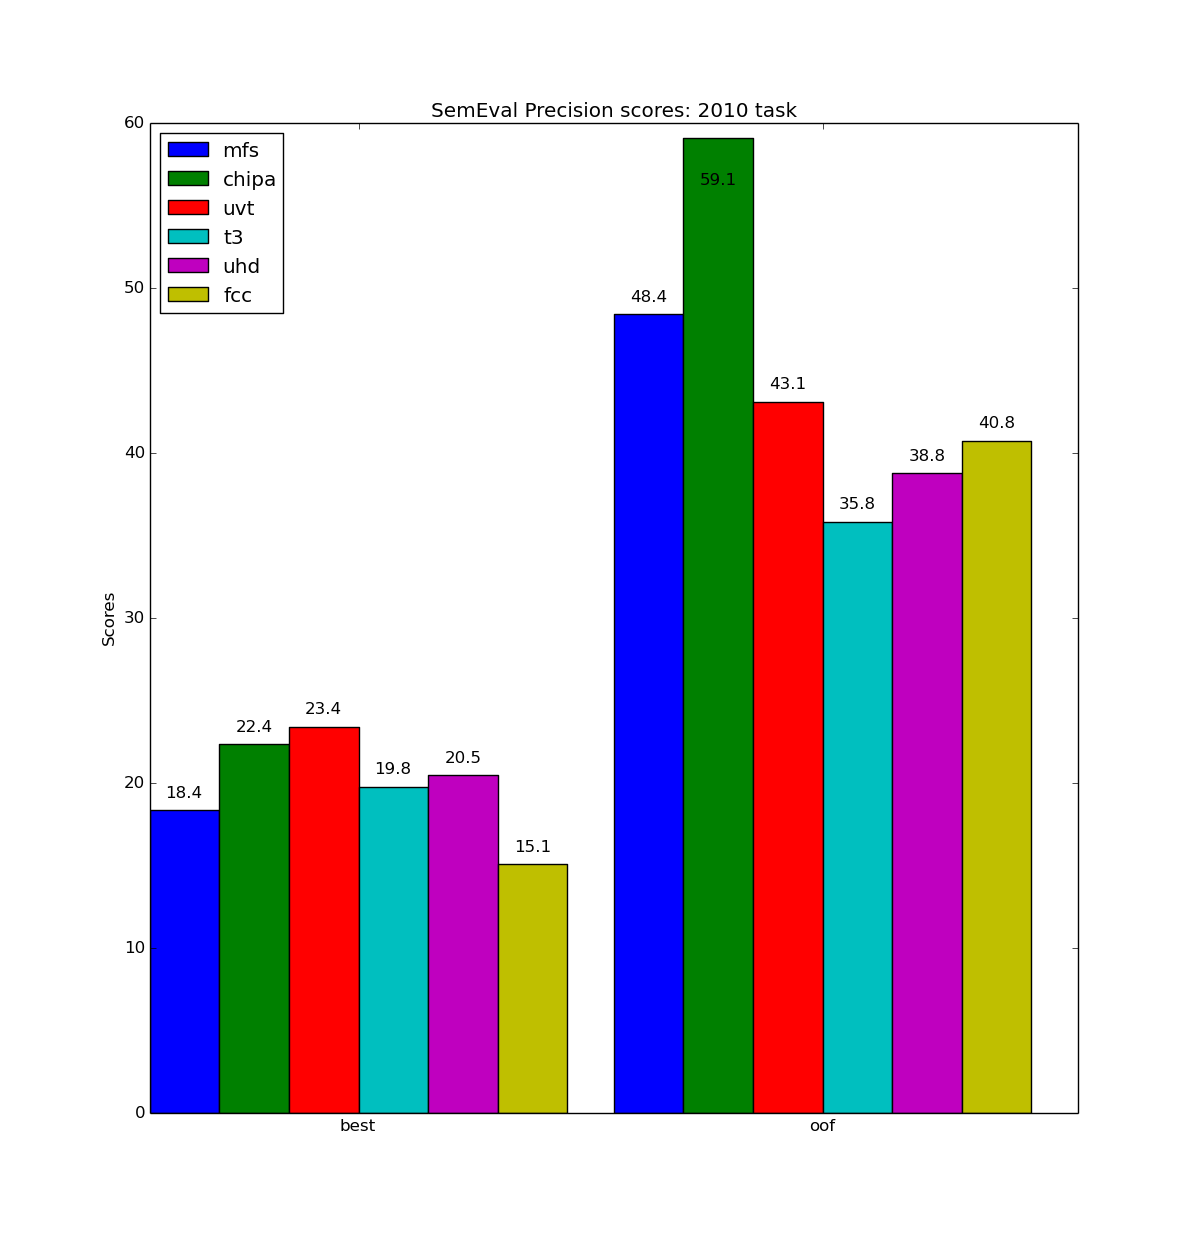
\includegraphics[width=\textwidth]{semeval-2010-ch4.png}
  \caption{Scores on the SemEval 2010 test set, including results posted in
  the shared task and the baseline Chipa system running on the same test set.}
  \label{fig:semeval2010:ch4}
\end{figure}

\begin{figure}
  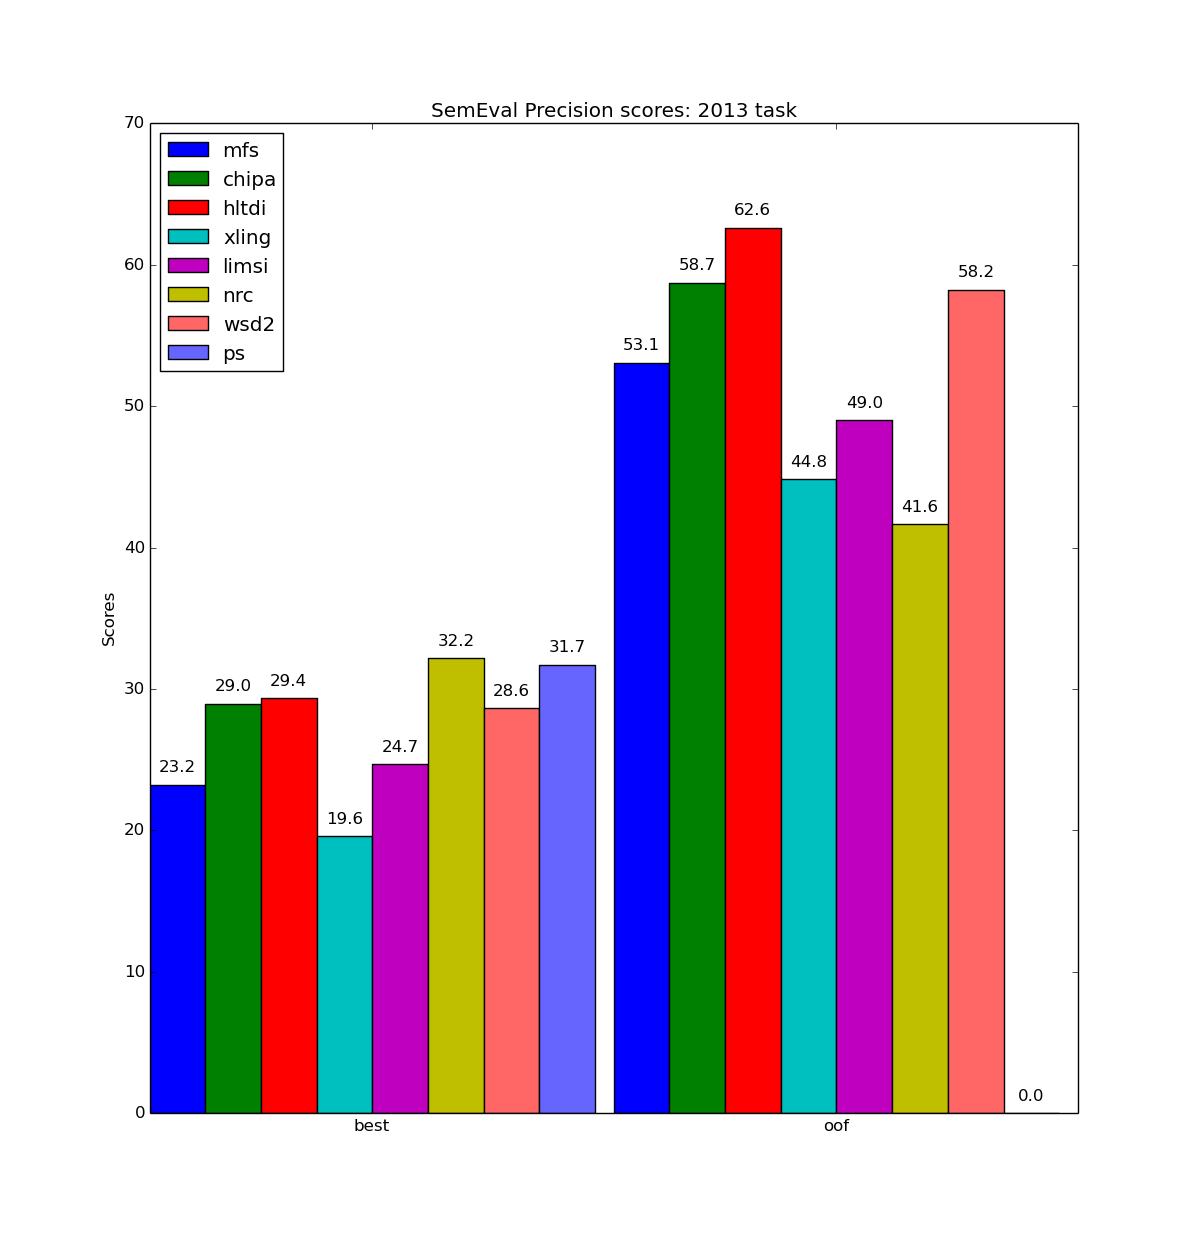
\includegraphics[width=\textwidth]{semeval-2013-ch4.png}
  \caption{Scores on the SemEval 2013 test set, including results posted in
  the shared task and the baseline Chipa system running on the same test set.
  When one team presented multiple results, here we take the best results from
  that team.}
  \label{fig:semeval2013:ch4}
\end{figure}

There were two settings for the evaluation, \emph{best} and \emph{oof}. In
either case, systems may present multiple possible answers for a given
translation, although in the \emph{best} setting, the first answer is given
more weight in the evaluation, and the scoring encourages only returning the
top answer.
In the \emph{oof} setting, systems are asked to return the top-five
most likely translations. In both settings, the answers are compared against
translations provided by several human annotators for each test sentence, who
provided a number of possible target-language translations in lemmatized form,
and more points are given for matching the more popular translations given by
the annotators. For a complete explanation of the evaluation and its scoring,
please see the shared task descriptions.

The scores for our systems are reported in Figure \ref{fig:semeval:theresults}.
In all of the settings, our systems posted some of the top results among
entrants in the shared task, achieving the best scores for some evaluations and
some languages.
For every setting and language, our systems beat the
most-frequent sense baseline, and our best results usually came from either the
L2 or MRF system, which suggests that there is some benefit in using
multilingual information from the parallel corpora, even without translating
the whole source sentence.

For the \emph{best} evaluation, considering only the mode gold-standard
answers, our L2 system achieved the highest scores in the competition for
Spanish and German. For the \emph{oof} evaluation, our MRF system -- with its
post-competition bug fix -- posted the best results for Spanish, German and
Italian in both complete and mode variants. Also, curiously, our L1 system
posted the best results in the competition for Dutch in the \emph{oof} variant.

For the \emph{best} evaluation, our results were lower than those posted by
ParaSense, and in the standard \emph{best} setting, they were also lower than
those from the \emph{c1lN} system \cite{maarten} and \emph{adapt1}
\cite{marine}.
This, combined with the relatively small difference between our simplest system
and the more sophisticated ones, suggests that there are many improvements that
could be made to our system; perhaps we could integrate ideas from the other
entries in the shared task this year.
